\chapter{Basic recon}
\label{chap:basic_recon}

As per usual when you get a box, the first step is to find as much information about it as you can. A quick \verb|nmap| reveals that port 80 and 22 are open. Http and ssh. Going to the ip in a browser shows a Magento webshop, with three items pre-configured. After some basic \gls{sqli} attempts, I decide that it's probably gonna be a bit more complex than that.

Then the hunt starts. The specs of the box say that \glspl{cve} are a big part of this box, so I start looking around for relevant \glspl{cve}. Not knowing what version of Magento is used, it was kind of a spray method. I noticed that the copyright was on 2014, so it's very likely that it's an older version.

There are two Magento versions, v1 and v2. I was still unsure what version was used, so I was just trying some exploits I could find. The exploits on \url{https://www.exploit-db.com/} turned out to be really useful, and it had a script (\#37977) to get a login on the admin dashboard. This script worked, and the admin page was on the default location (\verb|10.10.10.140/index.php/admin|).

\begin{figure}[H]
	\centering
	\captionsetup{justification=centering}
	\noindent 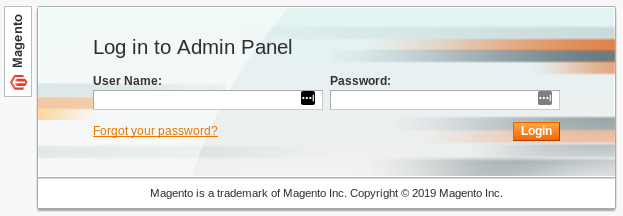
\includegraphics[width=\textwidth]{figures/magento-login.png}
	\caption{\emph{The login page of Magento}}
	\label{fig:magentologin}
\end{figure}

The admin page turned out to contain the version number of Magento, \verb|v|. This meant I could pin my exploit search to a specific version. After searching through the \gls{cms} for quite some time for interesting ways in, I was unsure where the exploit would be.

\vspace{5mm}

There was a lot written about exploiting a downloader included in Magento, but, after some reading on the HTB forums, I found out that this downloader was disabled because it was an unintentional way in.

Then I looked at exploit \#37811, hoping this would be it. I found\\ \verb|http://10.10.10.140/app/etc/local.xml|, giving me the install date, which could be used in the script. However, after running, with some slight modifications I got it to a point where it would crash with the error seen in \cref{fig:37811.py}. Searching for this error actually brings up the HTB forums for this challenge, stating that I should stop looking. It was apparently not the way forward.

\begin{figure}
	\centering
	\captionsetup{justification=centering}
	\noindent 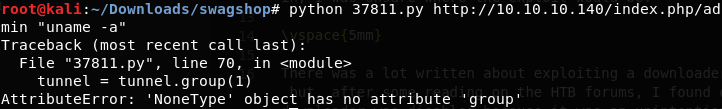
\includegraphics[width=\textwidth]{figures/python-37811-tunnel-error.png}
	\caption{\emph{The python script crashing}}
	\label{fig:37811.py}
\end{figure}